\section{Applikation}
I følgende afsnit bliver der gennemgået design, brugergrænseflade og implementering for User Stories for 'Login', 'Project List', 'Registrering på PDF' og 'Opret Bruger'. For den fulde dokumentation af design og implementering henvises til Arkitektur og Design dokumentationens Afsnit \ref{Design-sec:ApplikationDesign} og de tilhørende afsnit.

I analysen blev der taget udgangspunkt i at applikationen skulle udvikles i Xamarin Forms \cite{Forms}. Der blev under udviklingen fundet begrænsinger i Forms framework. Derfor er applikationen implementeringet i Xamarin iOS.

Til udvikling af Rambøll Tilsyn er der brugt et MVC design \cite{MVC}, som vist herunder, på Figur \ref{fig:MVC}. For beskrivelsen af MVC patternet henvises til Arkitektur og Design dokumentationens afsnit \ref{Design-sec:ApplikationDesign}.
\begin{figure}[H] % (alternativt [H])
	\centering
	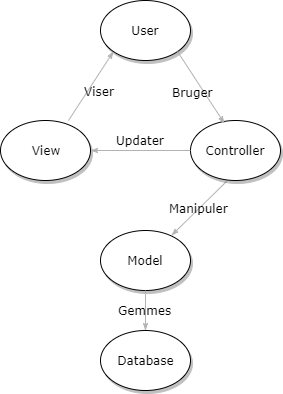
\includegraphics[height=12cm, width=10cm]{Design/Applikation/MVC}
	\caption{MVC design for Rambøll Tilsyn.}
	\label{fig:MVC}
\end{figure}

\clearpage

\section{Login}

\begin{figure}[H] % (alternativt [H])
	\centering
	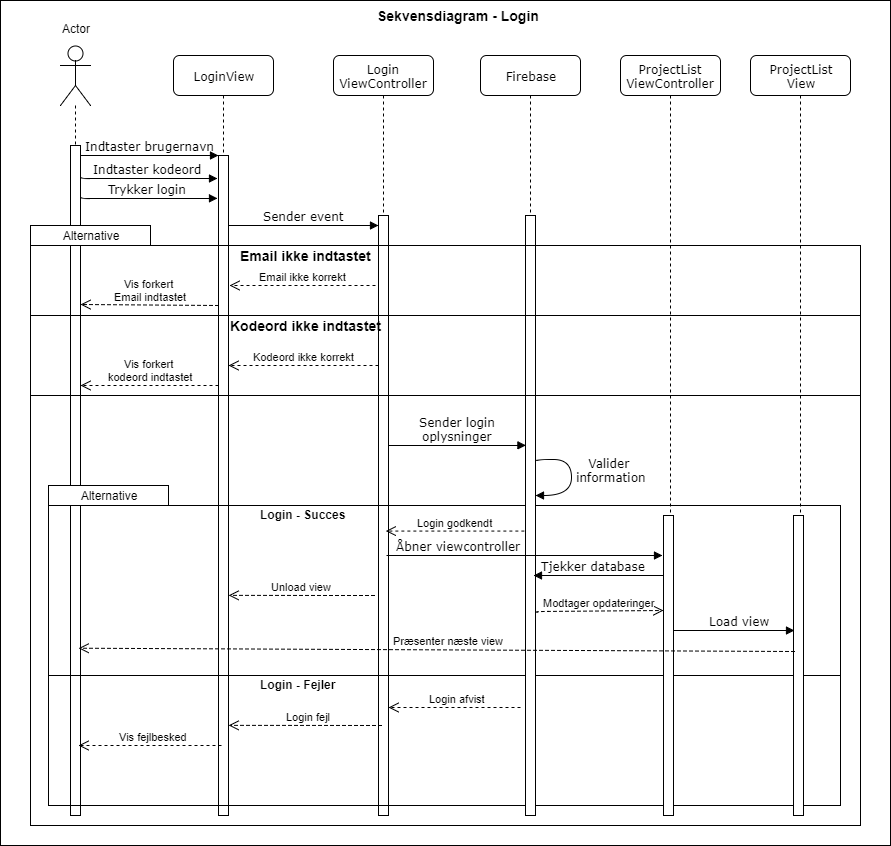
\includegraphics[width=1.1\textwidth]{../ArkitekturDesign/Design/Login/LoginSekvensDiagram}
	\caption{Sekvensdiagram for Login i Rambøll Tilsyn.}
	\label{fig:LoginSekvens}
\end{figure}
\subsection{Projekt oversigt}
I dette afsnit vises design, brugergrænseflade, implementering og test for 'ProjectList' viewet. For den fulde dokumentation henvises til Arkitektur og Design dokumentationens afsnit \ref{Design-sec:Opretbruger}.

\subsubsection{Design}
På Figur \ref{fig:ProjctListSekvens} ses sekvensdiagrammet for 'Project List' viewet til Rambøll Tilsyn.
\begin{figure}[H] % (alternativt [H])
	\centering
	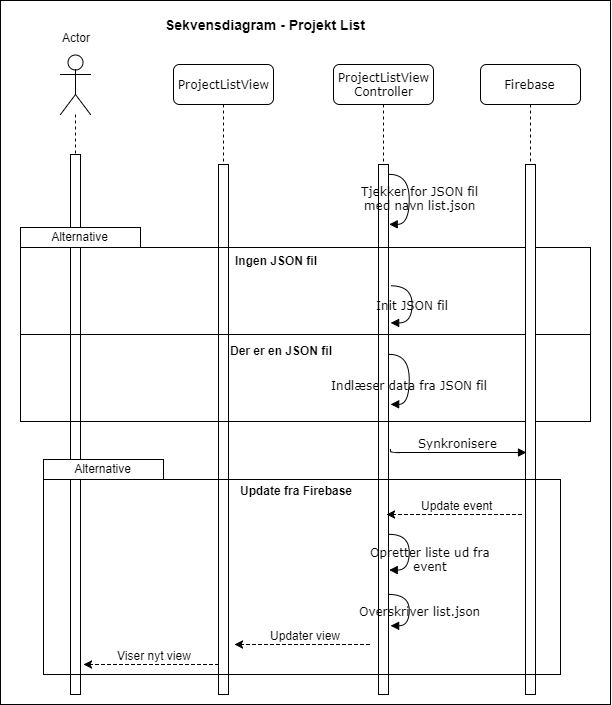
\includegraphics[height=15cm, width=12cm]{../ArkitekturDesign/Design/ProjectList/ProjektListSekvensDiagram}
	\caption{Sekvensdiagram for ProjectList i Rambøll Tilsyn.}
	\label{fig:ProjctListSekvens}
\end{figure}

\clearpage

\subsubsection{Grafisk brugergrænseflade}
I ProjectListViewet er der en oversigt over hvilke projekter der ligger i databasen, samt mulighed for tilføje projekt eller tilføj bruger. Se figur \ref{fig:ProjectListView}
\begin{figure}[H] % (alternativt [H])
	\centering
	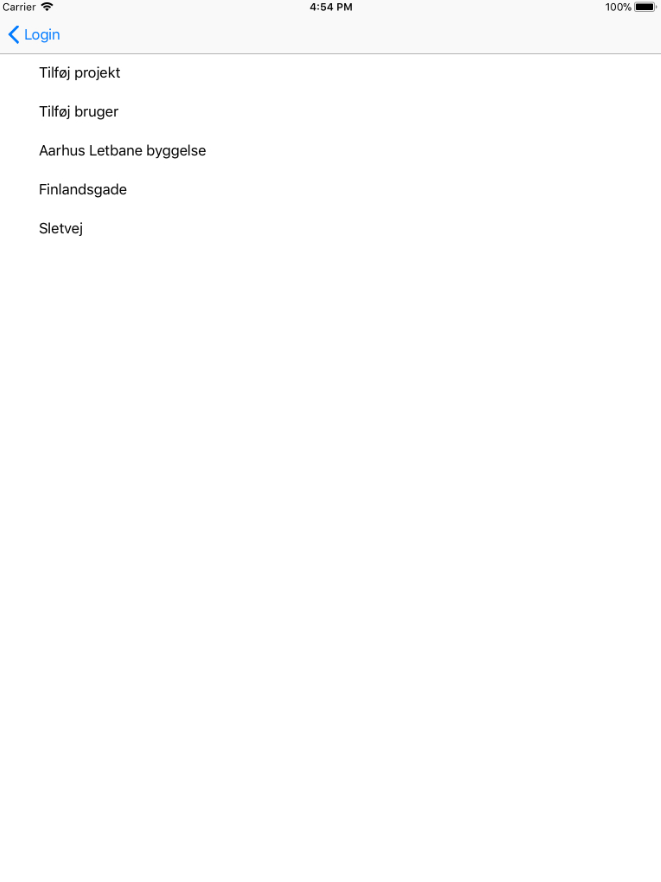
\includegraphics[height=12cm, width=10cm]{Design/Applikation/ProjektList/ProjectList}
	\caption{Project List viewet, som det er implementeret i Rambøll Tilsyn.}
	\label{fig:ProjectListView}
\end{figure}

\subsubsection{Implementering}
Før listen af projekter bliver vist for brugeren, initialiserer 'Project List' viewet en forbindelse til Firebase, hvor at den sætter et synkroniseringsevent, som kaldes såfremt der sker ændringer i PDF-filerne. \\
Dernæst opretter den en JSON-fil som indeholder alt projekt information fra Firebase. \\
Controlleren opretter nu et nyt TableView som har sourcen TableSource. Her laver den en liste bestående af alle projekter og muligheden for at tilføje bruger og tilføje projekt. \\
For en mere deltajeret beskrivelse af implementeringen og kode snips, henvises til Arkitektur og Design dokumentations afsnit \ref{Design-sec:ProjectList}.

\clearpage
\subsection{Registrering på PDF}
I dette afsnit vises design, bruger grænseflade, implementering og test for 'Registrering på PDF' viewet. For den fulde dokumentation henvises til Arkitektur og Design dokumentationens afsnit \ref{Design-sec:PDF}.
\subsubsection{Design}
Sekvensdiagrammerne for registrering på PDF tegning, er opdelt i tre for at overskueligegøre flowet. \\
Det første sekvensdiagram viser hvordan applikationen loader PDF tegningen ind. Sekvensdiagrammet kan ses på figur \ref{fig:LoadPDFSekvensDiagram}.
\begin{figure}[H] % (alternativt [H])
	\centering
	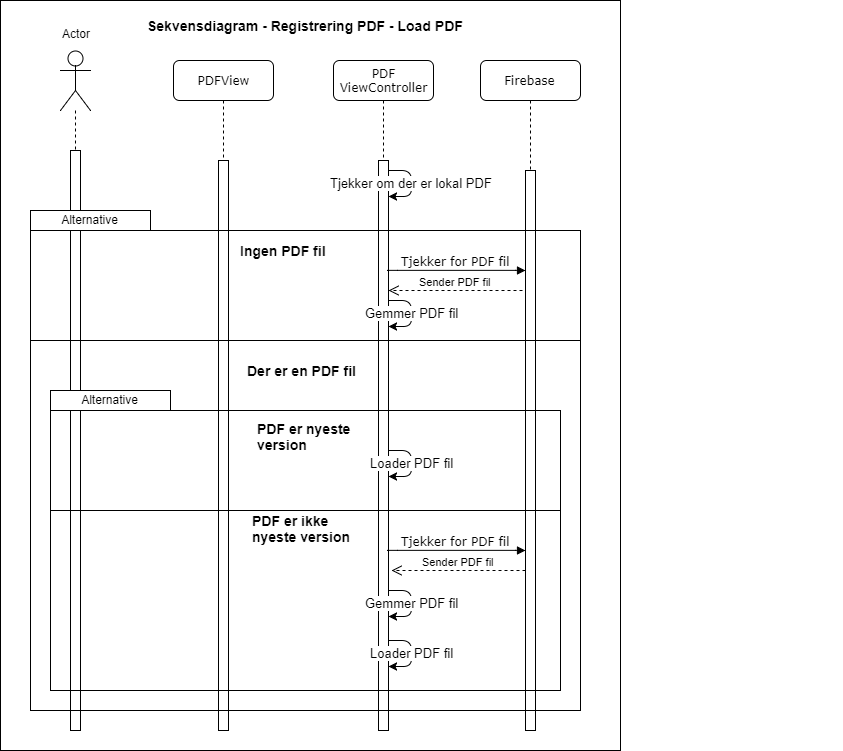
\includegraphics[height=12cm, width=15cm]{Design/Applikation/RegistrePDF/LoadPDFSekvensDiagram}
	\caption{Sekvensdiagram for Registrering på PDF - Loading af PDF, i Rambøll Tilsyn.}
	\label{fig:LoadPDFSekvensDiagram}
\end{figure}

\clearpage

Andet sekvensdiagram iser hvordan JSON filen bliver oprettet. Sekvensen med JSON sker direkte efter at PDF sekvensen er overstået. Sekvensdiagrammet kan ses på figur \ref{fig:LoadJSONSekvensDiagram}.
\begin{figure}[H] % (alternativt [H])
	\centering
	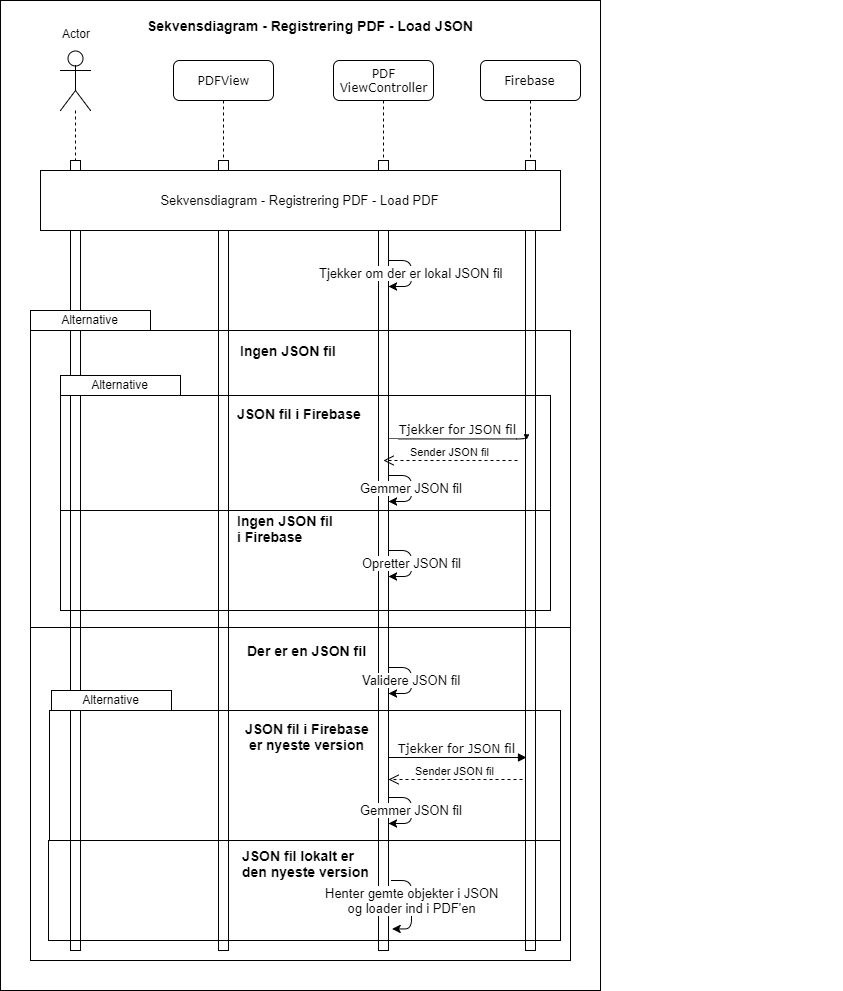
\includegraphics[height=15cm, width=15cm]{Design/Applikation/RegistrePDF/LoadJSONSekvensDiagram}
	\caption{Sekvensdiagram for Registrering på PDF - Loading af JSON, i Rambøll Tilsyn.}
	\label{fig:LoadJSONSekvensDiagram}
\end{figure}

\clearpage

Sidste sekvensdiagram, som sker i forlængelse af først Loading af PDF og Load JSON, viser hvordan systemet agere, når brugeren interagere med applikationen i forbindelse med oprettelse af objekter på PDF tegningen. Sekvensdiagrammet for dette kan ses på \ref{fig:RegistrerObjekterSekvensDiagram}.
\begin{figure}[H] % (alternativt [H])
	\centering
	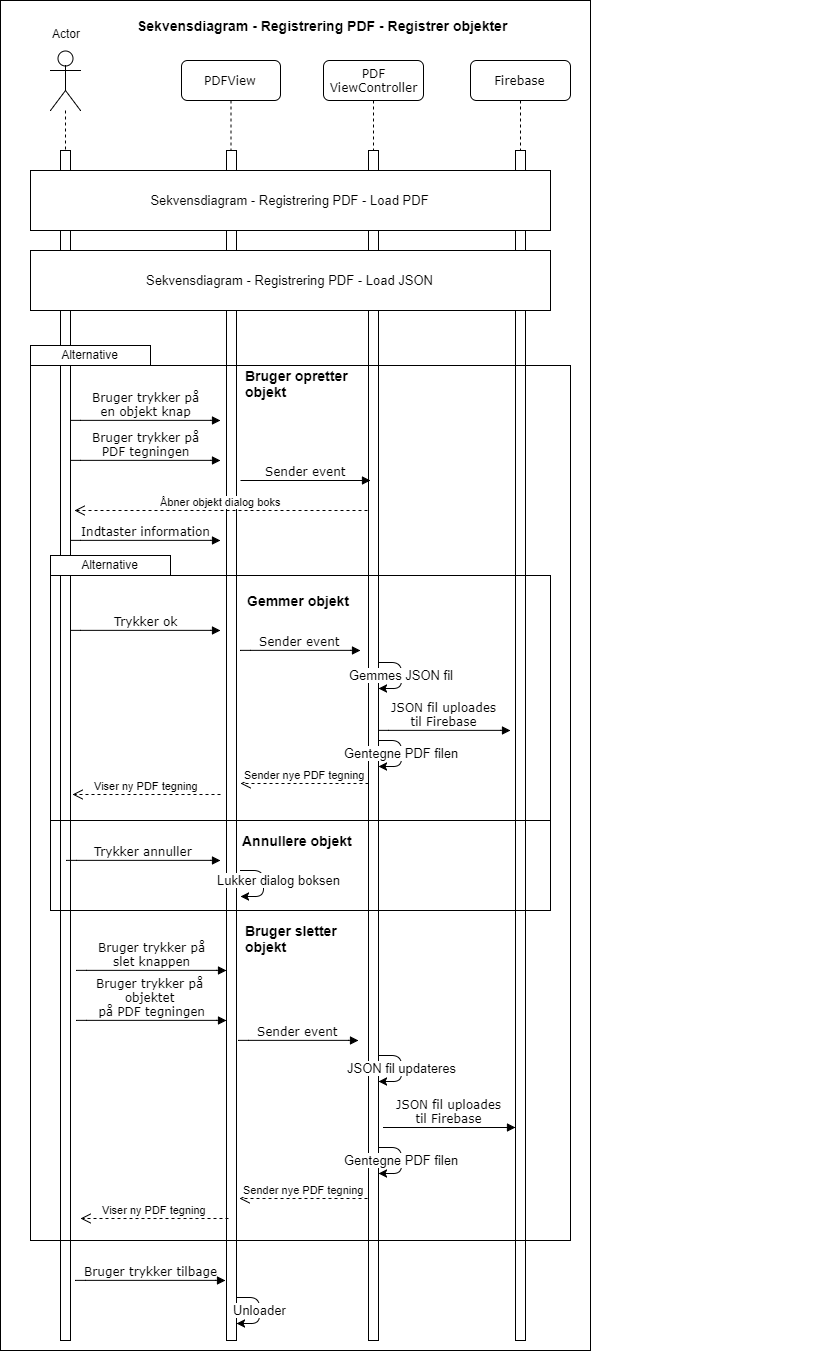
\includegraphics[height=18cm, width=15cm]{Design/Applikation/RegistrePDF/RegistrerObjekterSekvensDiagram}
	\caption{Sekvensdiagram for Registrering på PDF - Registrer på PDF, i Rambøll Tilsyn.}
	\label{fig:RegistrerObjekterSekvensDiagram}
\end{figure}

\clearpage

\subsubsection{Grafisk brugergrænseflade}
Grænsefladen for 'Registrer på PDF' viewet som ses på figur \ref{fig:RegistrerObjekterView} består af to views. 
Det øverste view viser PDF'en som tilhører projektet. \\
Det nederste view indeholder knapper som brugeren kan interagere med. Der er seks forskellige knapper: \\
De første to er frem og tilbage, hvor brugeren kan bladre mellem de forskellige sider i PDF'en. De tre knapper der kommer efter, er de symboler som brugeren kan tegne på PDF'en, ved at trykke på knappen og derefter det sted på PDF'en han ønsker. \\
Sidste knap er en liste knap. Her har brugeren mulighed for at afslutte sin registrering.
\begin{figure}[H] % (alternativt [H])
	\centering
	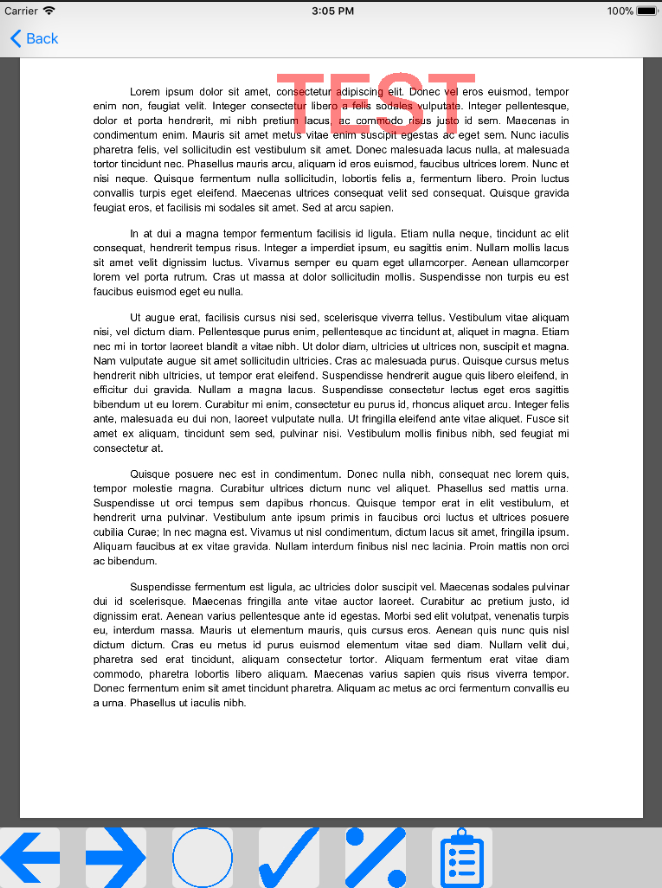
\includegraphics[height=12cm, width=10cm]{Design/Applikation/RegistrePDF/PDF}
	\caption{'Registrer på PDF' viewet som det er implementeret i Rambøll Tilsyn.}
	\label{fig:RegistrerObjekterView}
\end{figure}

\subsubsection{Implementering}
Når der navigeres ind i 'Registrering på PDF' viewet, loades PDF'en fra Firebase og gemmes lokalt. Den loades herefter ind i viewet. Efterfølgende oprettes et UIView hvor at symbol knapperne oprettes i. Når begge dele er oprettet og loadet, hentes information fra den JSON filen der blev hentet i 'Project List' viewet, og tegner så de objekter som er gemt i PDF'en. \\
Når disse er tegnet vises PDF'en for bruger. \\
For en mere deltajeret beskrivelse af implementeringen og kode snips, henvises til Arkitektur og Design dokumentations afsnit \ref{Design-sec:PDF}.


\clearpage
\section{Accepttest for Opret bruger (CRS-2)}
Dette afsnit beskriver accepttesten for Opret bruger.

\textbf{User story beskrivelse} \\
Som bruger \\
Ønsker jeg at kunne oprette en bruger på applikationen \\
For at kunne give en anden bruger adgang til systemet

\begin{table}[H]
	\centering
	\begin{tabular}{|ll|l|ll|} \hline
		\textbf{Scenarie} &  & \textbf{Beskrivelse}&  \textbf{Godkendt}&  \\ \hline
		Opret bruger&  &  Når alt information omkring en bruger &  OK&  \\
		& & er udfyldt, og der trykkes opret bruger, bliver brugeren oprettet& & \\ \hline
	\end{tabular}
	\caption{Accepttest for Opret bruger (CRS-2)}
	\label{AcceptOpretBruger}
\end{table}

\clearpage
